%-------------------------------------------------------------------------------
% seq64_meta_events
%-------------------------------------------------------------------------------
%
% \file        seq64_meta_events.tex
% \library     Documents
% \author      Chris Ahlstrom
% \date        2017-07-23
% \update      2017-07-23
% \version     $Revision$
% \license     $XPC_GPL_LICENSE$
%
%     Provides a discussion of the MIDI GUI meta_events that Sequencer64
%     supports.
%
%-------------------------------------------------------------------------------

\section{Sequencer64 Meta Event / SysEx Support}
\label{sec:meta_events}

   In recent versions of \textsl{Sequencer64} we are attempting better support
   for MIDI Meta and System Exclusive events, as well as a Tempo track.
   At present (v. 0.93.1), \textsl{Sequencer64} now supports the display of Set
   Tempo and Time Signature events.  They can also be added and edited, though,
   in this version, only in the event editor
   see \sectionref{sec:seq64_event_editor}.
   Furthermore, at this time only the first Tempo and Time Signature events are
   used to modify playback.
   System Exclusive support is also still in progress.
   So, currently, the most important feature is that they can be displayed.

   This section consolidates the description of the meta-event support.
   The following topics apply:

   \begin{enumerate}
      \item Tempo display min/max in "usr" settings.
      \item Tempo display in main window.
      \item Tempo display in pattern editor.
      \item Tempo display in song editor.
      \item Tempo and Time signature display and editing in the event editor.
   \end{enumerate}

   Before we discuss these items, we need to note how the tempo track is
   implemented in \textsl{Sequencer64}.  Rather man make a SeqSpec track for
   the tempo events, we follow the MIDI specification, which mandates that
   Tempo events must occur only in the first track.  \textsl{Sequencer64} has
   been upgraded so that Set Tempo and Time Signature events are full-fledged
   MIDI events and can be viewed (and later, edited) in the existing
   user-interface elements.  Notes and other events can occur in the same
   track, if the user-musician so desires.

\subsection{"usr" BPM Display Settings}
\label{subsec:meta_events_usr}

   \textsl{Sequencer64} allows the tempo to range from 1 to 600 BPM
   (beats per minute).    This range is hardwired into the application.
   But we need to be able to display tempo with a little more granularity.
   Therefore, \textsl{Sequencer64} provides some scaling for the tempo
   displays.  These values are found in the "usr" file:

   \begin{verbatim}
		0         # midi_bpm_minimum
		360       # midi_bpm_maximum
   \end{verbatim}

   See \sectionref{subsec:seq64_usr_file_user_midi_settings}, for more
   information.  These settings can only be made by editing the "usr" file
   while \textsl{Sequencer64} is not running.

\subsection{BPM Display in a Main Window Pattern slot}
\label{subsec:meta_events_mainwid_slot}

The following figure shows a note and some tempo changes.

\begin{figure}[H]
   \centering 
   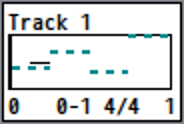
\includegraphics[scale=1.0]{meta/mainwid_pattern_tempo.png}
   \caption{Tempo in Pattern Slot}
   \label{fig:meta_events_mainwid_slot}
\end{figure}

The tempo is shown as a dashed cyan-colored line at the relative for the tempo,
based on the minimum and maximum values configured in the "usr" file as
discussed in the previous section.
This display is rudimentary.  It doesn't allow for ramping of the tempo at
present, and cannot be directly edited.

On the books for an upcoming version is to add a "tempo record" button that
enters the currently-set tempo into the pattern.

% \subsubsection{MIDI Metrics, PPQN}
% \label{subsubsec:meta_events_midi_ppqn}


%-------------------------------------------------------------------------------
% vim: ts=3 sw=3 et ft=tex
%-------------------------------------------------------------------------------
